\documentclass[a4paper,12pt]{article}

\usepackage[utf8]{inputenc}
\usepackage{newunicodechar}
\usepackage{float}
\usepackage[utf8]{inputenc}
\usepackage{newunicodechar}
\usepackage{titlesec}
\usepackage{textcomp}
\usepackage{enumitem}
\usepackage{amsmath}
\usepackage{ragged2e}
\usepackage{cancel}
\usepackage{titling}
\usepackage{amssymb}
\usepackage[rmargin=1.5cm,lmargin=2.5cm,tmargin=1.5cm,bmargin=1.5cm]{geometry}
\usepackage{hyperref}
\usepackage{tikz}
\usepackage{graphicx}
\usepackage{caption}
\usepackage{subcaption}
\usepackage{pythonhighlight}
\graphicspath{ {./images/} }
\newcommand*\circled[1]{\tikz[baseline=(char.base)]{
            \node[shape=circle,draw,inner sep=2pt] (char) {#1};}}
\newcommand{\ans}[1]{\boldsymbol{\underline{#1}}}
\newcommand{\textans}[1]{\textbf{\underline{#1}}}
\newcommand{\vm}[1]{\begin{vmatrix}#1\end{vmatrix}}
\newcommand{\vb}[1]{\begin{bmatrix}#1\end{bmatrix}}
\newcommand{\m}[1]{\mathbb{#1}}
% \newcommand{\suct}[3]{\chapter{\textbf{#1} #2}#3}
\newcommand{\enum}[1]{\begin{enumerate}[label=\alph*)]#1\end{enumerate}}
\newcommand{\numenum}[1]{\begin{enumerate}[label=\arabic*.]#1\end{enumerate}}

\DeclareRobustCommand{\[}{\begin{equation}}
\DeclareRobustCommand{\]}{\end{equation}}

\usepackage{setspace}
\setlength{\parindent}{1cm}
\onehalfspace

\usepackage{fontspec}
\usepackage{algorithm} 
\usepackage{algpseudocode}
 
\setmainfont[SizeFeatures={Size=14}]{Times New Roman}
\numberwithin{equation}{section}
\numberwithin{algorithm}{section}
\counterwithin{figure}{subsection}

\title{Kinodynamic Motion Planning}
\author{}
\begin{document}


\section{Abstract}

Autonomous navigation systems usually include a path planner and a local planner.
The first one provides a somewhat kinematically reasonable path, which often cannot be passed by a robot,
while the second one tries to adapt the path to the dynamic environment and other constraints that were not checked by the path planner.
This work is an attempt to create an optimized RRT-based path planner that takes into account nonholonomic constraints.
This is achieved through an analysis and combination of already existing solutions, usage of R-Trees, techniques like goal-biased sampling and more. As a result, open source reference implementation in Python constructs trees that require far less local (reactive) planning than typically.
\subsection{Keywords}{}{}\hfill

Path planning, Collision avoidance, Nonholonomic constraints, Rapidly exploring Random Tree, R-Tree, Reeds-Shepp Car.

\section{Introduction}

Motion planning and autonomous vehicles have been developing for quite long time already and in recent 20 years those areas have grown
from enterprise-only solutions (i.e. robotic arms and other manufacturing devices) to consumer-friendly ones (robot vacuums and "autopilots" in cars).
If initially the problem was to "get from point A to point B", by this time it has been expanded with operation in dynamic environments, collision avoidance, computation efficiency and others.

All of the mentioned problems have one thing in common - Configuration Spaces framework that is used to describe the
state of the robot in the environment. In order to state the problem one should define C-Space - $\mathcal{C}$, which includes configurations of the robot $q$, world $\mathcal{W}$ (including obstacles) and other constraints.

This work is aimed to solve the problem of planar path-planning, thus $\mathcal{W}=\mathbb{R}^2$. Some parts of the world are occupied by the obstacles $\mathcal{O}\subset\mathcal{W}$ defined by polygons, which cannot be self-intersecting. And finally the robot - a rigid body $\mathcal{A}$,
which can translate in the world, making $\mathcal{C}$ a manifold $M_1=\mathbb{R}^2$, and rotate around its bounding box center, which adds $M_2=\mathbb{S}^1$, thus without obstacles:
\[
\mathcal{C}=\mathbb{R}^2\times\mathbb{S}^1=SE(2)
\]

The robot's configuration in the space is defined as a vector $q=(x,y,\theta)$ and the space that it is occupying as $\mathcal{A}(q)\subset\mathcal{W}$.
Thus, the configuration space for obstacles is:
\[
\mathcal{C}_{obs}=\{q\in\mathcal{C}\mid\mathcal{A}(q)\cap\mathcal{O}\neq\emptyset \}\hspace{5pt}[1]
\]
\[
\mathcal{C}_{free}=\mathcal{C}\setminus\mathcal{C}_{obs}
\]

The algorithm is created with holonomic - the robot can only travel in $\mathcal{C}_{free}$ - and nonholonomic constraints in mind - it uses Reeds-Shepp Car model and steering function as the only way to produce a path from $q_1\in\mathcal{C}_{free}$ to $q_2\in\mathcal{C}_{free}$, making some configurations in $C_{free}$ unreachable. The Reeds-Shepp Car has only two gears - forward and reverse ($u\in\{-1,1\}$); and angular velocity that depends on maximum turning radius with unit-velocity $r_{turn}$ - $w = \frac{v=1}{r_{turn}}$. In general, the path would be a non-linear function of time, as a turn is a curve. However, in order for a robot to be able to follow the path, each turn is approximated with a given level of discretization $\delta$ to a set of straight lines:

\[
\begin{cases}
\dot{x}=x_{prev} + u\cdot\delta\cdot\cos{\theta}\\
\dot{y}=y_{prev} + u\cdot\delta\cdot\sin{\theta}\\
\dot{\theta}=\theta_{prev}+u\cdot \frac{\delta}{r_{turn}}
\end{cases}
\]

Finally, the starting points are defined as $q_i\in\mathcal{C}_{free}$ and the goal point is $q_g\in\mathcal{C}_{free}$. The local planner should produce a path, which is a set of connected linearized curves that were provided by the steering function.

Generally, industry solves such problem with either a "sampling" algorithm (RRT and variants, PRM) or a graph traversal algorithm like A*. Right now RRT-like algorithms are used more as with a proper set of improvements they can converge quite fast. Classical implementation comes with two parameters - iterations limit $K$ and maximum edge length $\Delta{t}$. The data on obstacles is often stored as points in KD-Tree and the collision detection is performed by querying it. Nonholonomic constraints are usually left to the reactive planner. There are several
drawbacks related to those approaches. Firstly, the use of KD-Tree implies a complexity increase on tree expansion, as KD-Tree is not meant to be updated [2]. Secondly, collision detection in such cases is often done by checking the area of some radius around the robot, which makes it impossible for a planner to create a path through narrow corridors, or by checking its bounding box, which is inefficient for any shape except for rectangles that are aligned to the axes (which is not true for any rotated rectangle). And finally, lack of nonholonomic constraints might make the whole path unreachable. The aim of the presented algorithm is not to suffer from those issues with as little overhead compared to others as possible.
This is achieved with the help of R-Tree, special polygon approximation technique, goal-biased sampling [3] and nearest neighbor randomization.

\section{Literature Overview}

All previous conclusions about "the industry" were obtained by analysing recent researches published at ICRA, IROS, IEEE and other robotics-related conferences.

Many researches in this field are focused on creating smooth and efficient pathplanning curves keeping environments quite restricted. That is, such environments often support only convex obstacles and robot shapes, while, for example, on a real parking lot various non-convex obstacles are possible (flowerbeds, sidewalks, etc.). Omur Arslan, Vincent Pacelli and Daniel E. Koditschek (2017) [4] suggest a way of significantly improving graph connectivity for sampling-based motion planning algorithms, but for convex obstacles and a car represented by a point. Sadhu, Arup Kumar, Shukla, Shubham, Bera, Titas, Dasgupta, Ranjan (2019) [5] contribute an algorithm able to find paths is environment with many obstacles, although simplifying car shape to a square box. Papers focusing on collision avoidance in dynamic environments (Jiahui Lin, Tong Zhou, Delong Zhu, Jianbang Liu, Max Q. H. Meng, 2020) [6] also suffer from simplified car models and radius-based collision check methods. Our work could improve these algorithms by making them more suitable for real life object configurations.


\section{The Proposed Method: BR-RRT}
Our method (BR-RRT - Box and R-Tree-RRT) is based on the RRT algorithm and essentially is an extension for it. The difference from other works lies in data structures,
point sampling approach and collision detection.

\subsection{Tree and Obstacles in R-Tree}

As the data structure for the tree points we propose R-Tree, which does not always require full tree rebuild for an insertion.
While R-Tree does not drastically differ in complexity terms from a KD-Tree, it has an advantage of being able to store not just vertices,
but spatial data in forms of rectangles.

Some works proposed the use of R-Trees as a structure for obstacles as well. However, in shaped that is not a rectangle and not perfectly aligned to the axes requires significantly
more $\mathcal{C}_{free}$ space than it actually should (Fig. 4.1.a). Since it can drastically decrease performance of the algorithm at turns, we are proposing an algorithm for
approximation of polygons to a set of axes-aligned rectangles. This kind of approximation of both obstacles and the car allows to store everything in the R-Tree. However, it would be more beneficial to store it in a differently configured R-Tree,
as density and amount of data points is incomparable to those in the RRT nodes tree.

\begin{algorithm}[H]
    \caption{Boxify}
    \begin{algorithmic}[1]
    \State Input $O$: Obstacle, $p$: detalization factor 
    \State $x_{min}$, $y_{min}$, $x_{max}$, $y_{max}$ = BoundingBox($O$)
    \If {$y_{max} - y_{min} < x_{max} - x_{min}$}
    \While {$y_{min} < y_{max}$}
    \State $y_{up}$ = min($y_{max}, y_{min}+p$)
    \State $O_{cut}$ = RectangleClip($O, x_{min}, y_{min}, x_{max}, y_{max}$)
    \State $y_{min} = y_{min} + p$
    \State yield $O_{cut}$
    \EndWhile
    \Else
    \While {$x_{min} < x_{max}$}
    \State $x_{up}$ = min($x_{max}, x_{min}+p$)
    \State $O_{cut}$ = RectangleClip($O, x_{min}, y_{min}, x_{max}, y_{max}$)
    \State $x_{min} = x_{min} + p$
    \State yield $O_{cut}$
    \EndWhile
    \EndIf
    \end{algorithmic}
\end{algorithm}

The function RectangleClip tries to find an intersection between the obstacle and given rectangle. Such function is defined and well optimized in various geometry engines (e.g. GEOS).

\begin{figure}[H]
\centering
    \begin{subfigure}[b]{0.4\textwidth}
        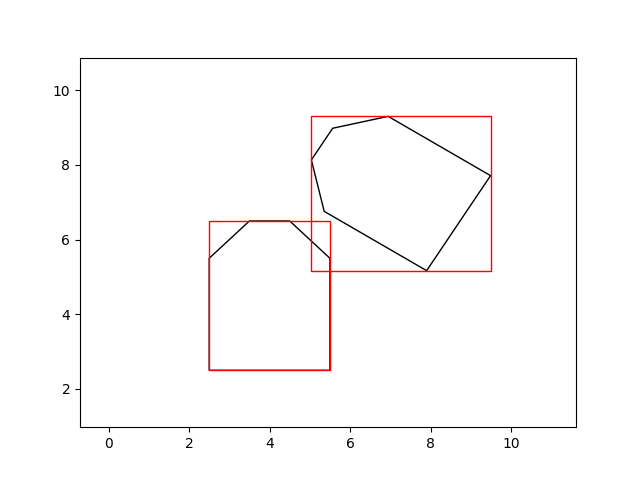
\includegraphics[scale=0.3,width=\textwidth]{images/car_bounding_box.png}
        \caption{Bounding box false collision}
    \end{subfigure}
    \begin{subfigure}[b]{0.4\textwidth}
        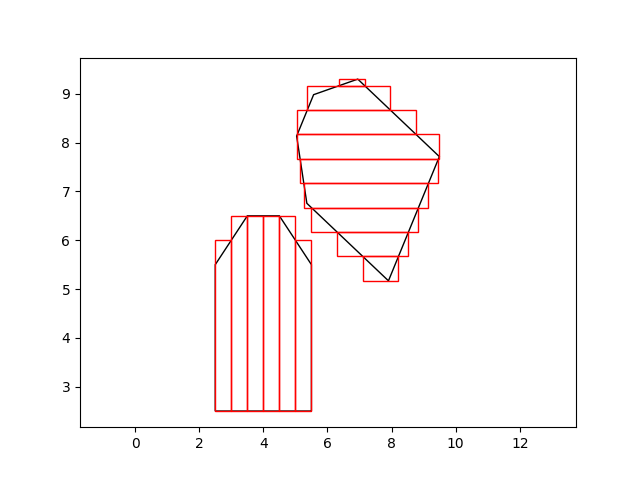
\includegraphics[scale=0.3,width=\textwidth]{images/car_boxify_0_5.png}
        \caption{Boxify p=0.5}
    \end{subfigure}
    \begin{subfigure}[b]{0.4\textwidth}
        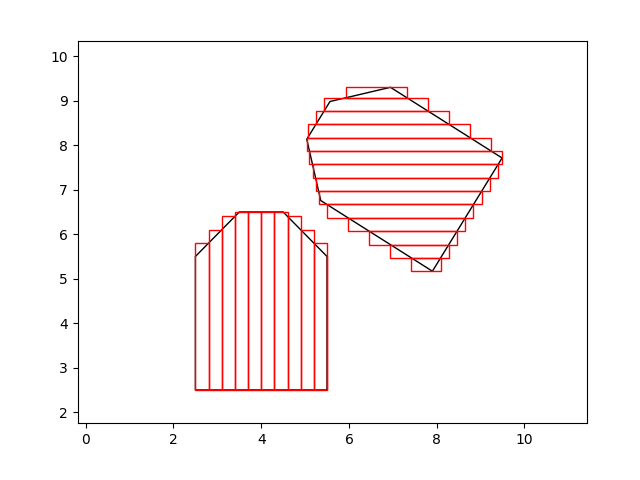
\includegraphics[scale=0.3,width=\textwidth]{images/car_boxify_0_3.png}
        \caption{Boxify p=0.3}
    \end{subfigure}
    \begin{subfigure}[b]{0.4\textwidth}
        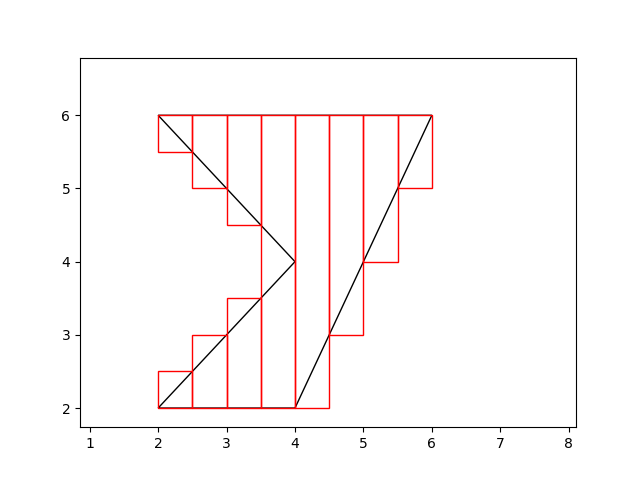
\includegraphics[scale=0.3,width=\textwidth]{images/concave_boxify.png}
        \caption{Boxify p=0.5}
    \end{subfigure}
    \captionsetup{width=0.6\textwidth}
    \caption{An example of inefficient collision check with bounding boxes compared to the proposed function with different parameter.}
\end{figure}

\subsection{Sampling}

By default, RRT algorithm picks a random point $q\in\mathcal{C}_{free}$ and tries to build a trajectory from the nearest point in the tree to it (at the first iteration the
nearest point is set to be $q_i$).
The way to determine that the point is reachable is usually constructing a straight line between the sample point and the existing one.
Then, if trajectory is built, the point is added the tree.

A common enhancement to this process is goal-biased sampling [3]. In this case, with a parameterized probability $g_r$ instead of choosing a random point in $C_{free}$. This approach, however,
has a flaw. If the tree has grown close to the $q_g$ with only one branch with last node $q_1$ and due to nonholomonic constraints cannot reach the $q_g$, all later samples that
were changed on $q_g$ will get trapped by $q_1$, which has minimal distance to the $q_g$, until a new point $q_2: dist(q_2, q_g) < dist(q_1, q_g)$ is added to the tree.
In order to increase the chances of "untrapping" the $q_g$, we propose the following: since after sampling a point or choosing the $q_g$ as the sample point the algorithm tries to 
find the nearest nodes already added to the tree, one could select a random node from the set of $n$-closest nodes without any computational drawback.

\begin{figure}[H]
\begin{center}
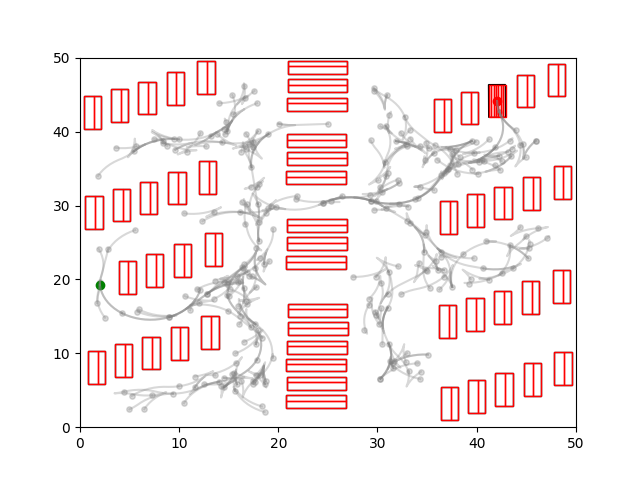
\includegraphics[scale=0.7]{images/car_trapped.png}
\captionsetup{width=0.6\textwidth}
\caption{An example of a vehicle nonholonomically trapped due to angular precision. It stands at the finish point in the wrong direction. RRT with goal sampling will fail to find a trajectory at each $q_g$ check.}
\end{center}
\end{figure}

Additionally, instead of computing Euclidean distances to all nodes, our algorithm queries the R-Tree on the closest neighbors and computes the Reeds-Shepp distance to them.
The final step of the sampling process involves checking feasibility of the provided trajectory.
For each point $q$ provided by the trajectory generator (steering function) the algorithm performs $Boxify(\mathcal{A}(q), p)$.
Other researches proposed converting $\mathcal{O}$ into TP-Space (Trajectory Parameter-Space) [7], which would represent an intersection of $\mathcal{C}_{free}$ and 
kinodynamically feasible trajectories available in $\mathcal{A}(q)$. However, this would strongly increase the dimension of the $\mathcal{C}_{free}$ and would require
storing nodes in the same dimension, which then would lead to higher complexity in the nearest neighbor queries on the RRT tree data structure.
In our implementation $\mathcal{C}_{free}$ stays in $SE(2)$ and the maximum number of collision checks $\mathcal{O}_{checks}$ depends on the amount of iterations $k$, RRT maximum edge length $\Delta{t}$, chosen shape approximation discretization factor $p$ and trajectory discretization factor $\delta$.
\[
\mathcal{O}_{checks} \leq k\cdot p\cdot \frac{\Delta{t}}{\delta}\label{eq:max_coll_checks}
\]

\begin{algorithm}[H]
    \caption{Complete BR-RRT}
    \begin{algorithmic}[1]
    \State Constants: R-Tree with obstacles $rt_{obs}$
    \State Environment and Car Inputs: $\mathcal{C}$, $q_i$, $q_g$, $precision$, $\mathcal{A}$
    \State Parameters Inputs: $\Delta{t}$, $K$, $g_r$, $p$, $\delta$, $n$
    \State $rt_{tree}$ = R-Tree$(g_i)$
    \For {$k$ in $1..K$}
        \If {$random(0, 1) > (1 - g_)$}
            \State $q_s$ = $q_g$
        \Else
            \State $q_s$ = $q_{rand}\in\mathcal{C}_{free}$
        \EndIf
        \State $nodes$ = NNQuery$(rt_{tree}, q_s, n)$
        \State $q_n$ = RandomChoice($nodes$)
        \State $path$ = Reeds-Shepp($q_n$, $q_s$)
        \For {$q$ in $path$}
            $boxes$ = Boxify$(\mathcal{A}(q))$
            \For {$box$ in $boxes$}
                \If {IntersectionQuery$(rt_{obs}, box) > 0$}
                    \State continue
                \EndIf
            \EndFor
        \EndFor

        \If {InGoalRegion$(q_n, q_g, precision)$}
            \State return $\text{Node}_s$
        \EndIf        

        \State $\text{Node}_n$ = GetNode$(q_n)$
        \State $\text{Node}_s$ = Node$\{position=q_s, root=\text{Node}_n, path=path\}$
        \State Add$(rt_{tree}, \text{Node}_s)$
    \EndFor
    \State return "Not enough iterations"
    \end{algorithmic}
\end{algorithm}

\subsection{Testing methodology}
\subsubsection{Car Model}

Since the research is conducted for car-like robots autopilots,
for testing purposes we have conducted a brief analysis of local car market and chose parameters of one of the best selling cars.

The polygonal model of the car is simplified to a rectangle, but the implementation can accept any polygonal object as a car,
and the algorithm was designed for complex-shaped cars. The model has the following parameters: $length=4.42m$, $width=1.7m$ and turning radius of $r_{turn}=5.12m$.

For the car model discretization factor $p$ of the Boxify algorithm was set to $0.25$, which means approximation to rectangles with smallest edge of at most $0.25cm$.
The position $q$ is defined by coordinates of the centroid of the car.

\subsubsection{Map Model}

For the map we have chosen an arbitrary parking problem that was designed to include complex scenarios. The parking ($50x50m$) is filled with same cars as our testing car.
Obstacle discretization factor $p$ is set to $p=1$ ($1m$).

\begin{figure}[H]
\begin{center}
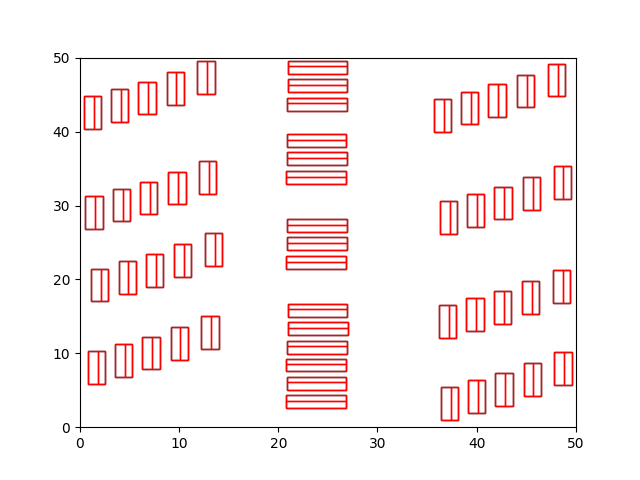
\includegraphics[scale=0.7]{images/large_map.png}
\captionsetup{width=0.6\textwidth}
\caption{Large parking model for conducting tests}
\label{fig:large_map}
\end{center}
\end{figure}

\subsubsection{Testing System}

Each algorithm was tested on multiple different values of all parameters. 
For each set of parameters the testing system chose two random cars-obstacles from the map, removed them and inserted $q_i$ and $q_g$ instead. The testing car was then
moved to $q_i$ and rotated accordingly. This environment setup was then passed to BR-RRT and the path was calculated along side with additional statistical data.
This process was repeated 100 times for each set of parameters in parallel. Due to parallel execution, in this particular testing there will not be any analysis of
absolute computation time. In general, since the reference implementation is written in Python and executed on a powerful machine
that might not be a good representation of robot's hardware, absolute values of time are not very useful.

\subsection{Baseline RRT Results}

For the baseline algorithm we have chose not a classical RRT, but an improved one.
This algorithm uses goal-biased sampling and the proposed Boxify method for the collision detection. The latter condition does not affect testing as it was enabled in all tests.

\begin{figure}[H]
\centering
    \begin{subfigure}[b]{0.6\textwidth}
        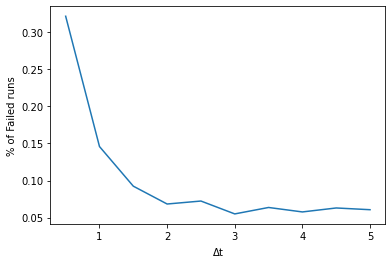
\includegraphics[scale=0.6,width=\textwidth]{images/baseline_failure_dist.png}
        \caption{Distribution grouped by $\Delta{t}$}
        \label{fig:baseline_edge_len_fail_dist}
    \end{subfigure}
    \begin{subfigure}[b]{0.6\textwidth}
        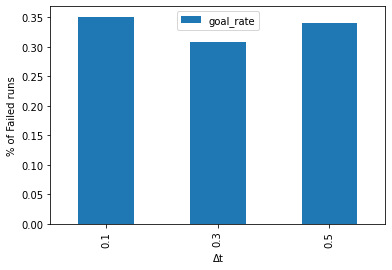
\includegraphics[scale=0.6,width=\textwidth]{images/baseline_failure_dist_grate.png}
        \caption{Distribution grouped by $g_r$}
    \end{subfigure}
    \caption{Distribution of failed runs in baseline RRT for different parameters}
\end{figure}

In the baseline RRT the maximum edge length, that can be added to the RRT tree, plays the most significant role in its completion rate [Fig. \ref{fig:baseline_edge_len_fail_dist}].
From the graph we observe that $\Delta{t}=0.5$ accounts for more than 30\% of fails. $\Delta{t}>=3.0$ shows the best results and can be considered as the best.
It is important to understand why it is so. RRT has a parameter of iterations limit. On a large map, like the one
that is shown at Fig. \ref{fig:large_map},
a path from a random $q_i$ to a random $q_g$ can be long even in Euclidean terms. If the $\Delta{t}$ is too small, the distance between $q_i$ and $q_g$ can be just greater than $K\cdot\Delta{t}$.
However, it still shouldn't be considered an artificial disadvantage of small $\Delta{t}$, because from Equation \ref{eq:max_coll_checks} we know that amount of iterations directly affect the amount of performed collision checks. In fact, Figure \ref{fig:baseline_iterations} shows that runs with low values of $\Delta{t}$ failed more often compared to others
and confirms previous conclusions. Similar results were obtained on other maps.

\begin{figure}[H]
\centering
    \begin{subfigure}[b]{0.6\textwidth}
        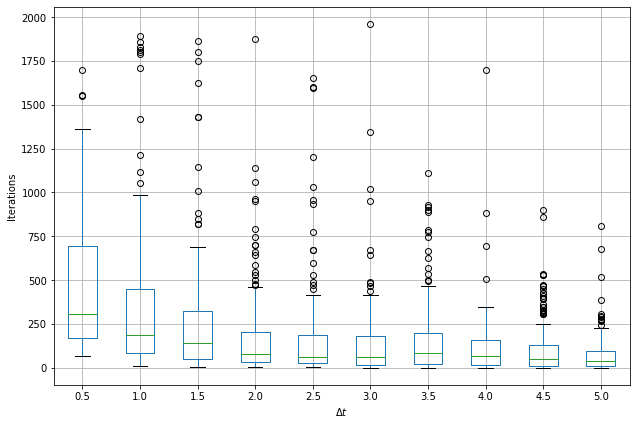
\includegraphics[scale=0.7,width=\textwidth]{images/baseline_low_distance_iterations_over_t.png}
        \caption{Euclidean Distance < 10m}
        \label{fig:baseline_edge_len_fail_dist}
    \end{subfigure}
    \begin{subfigure}[b]{0.6\textwidth}
        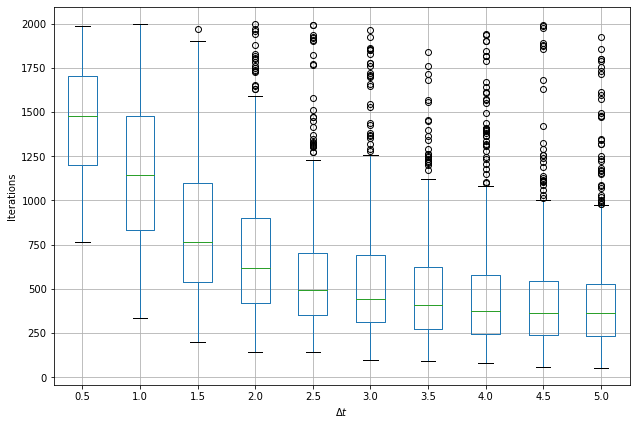
\includegraphics[scale=0.7,width=\textwidth]{images/baseline_high_distance_iterations_over_t.png}
        \caption{Euclidean Distance > 35m}
    \end{subfigure}
    \caption{Baseline RRT Iterations distributions for different values of $\Delta{t}$}
    \label{fig:baseline_iterations}
\end{figure}

\subsection{BR-RRT Results}

Our algorithm was tested in similar methodology, however, one parameter was added - $n$ for the randomized nearest neighbor approach. 
Case of $n=1$ must be same in output as Baseline RRT, as the only difference then is the data structure under the hood. From Figure \ref{fig:brrrt_iters_low} we can see
that increasing the number $n$ tends to decrease the number and the variance of the number of iterations at low distances. Difference between values 3 and 6 is not that
substantial. However, low distances tend to vary more in terms of actual distance to the goal. Figure \ref{fig:brrrt_iters_high} that illustrates iterations at high distances
has much clearer trend that leads to the same conclusions. The number of outliers there is higher, but the number of sample is higher too. 

\begin{figure}[H]
\centering
    \begin{subfigure}[b]{0.6\textwidth}
        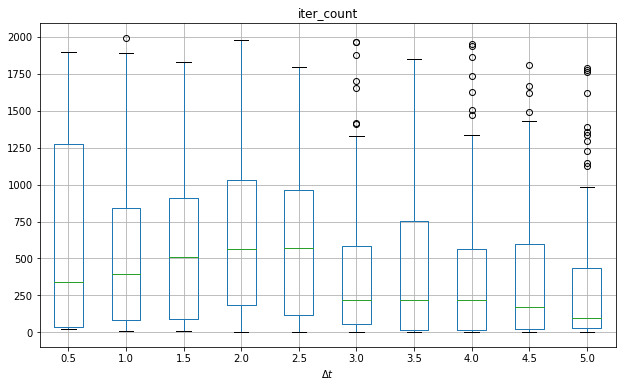
\includegraphics[scale=1,width=\textwidth]{images/brrrt_iters_low_n_1.png}
        \caption{Euclidean Distance < 10m, n=1}
        \label{fig:baseline_edge_len_fail_dist}
    \end{subfigure}
    \begin{subfigure}[b]{0.6\textwidth}
        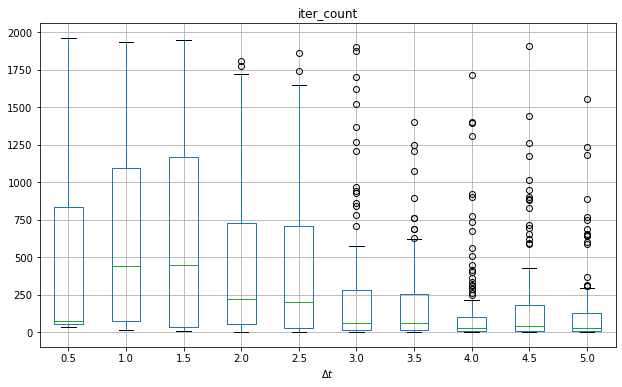
\includegraphics[scale=1,width=\textwidth]{images/brrrt_iters_low_n_3.png}
        \caption{Euclidean Distance < 10m, n=3}
    \end{subfigure}
    \begin{subfigure}[b]{0.6\textwidth}
        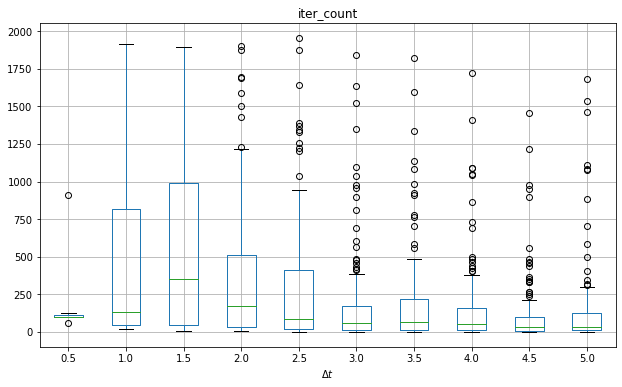
\includegraphics[scale=1,width=\textwidth]{images/brrrt_iters_low_n_6.png}
        \caption{Euclidean Distance < 10m, n=6}
    \end{subfigure}
    \caption{BR-RRT Iterations distributions for different values of $\Delta{t}$ and $n$.}
    \label{fig:brrrt_iters_low}
\end{figure}

\begin{figure}[H]
\centering
    \begin{subfigure}[b]{0.6\textwidth}
        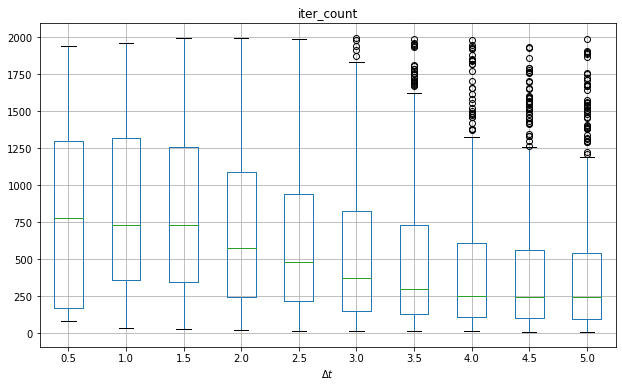
\includegraphics[scale=1,width=\textwidth]{images/brrrt_iters_high_n_1.png}
        \caption{Euclidean Distance > 30m, n=1}
        \label{fig:baseline_edge_len_fail_dist}
    \end{subfigure}
    \begin{subfigure}[b]{0.6\textwidth}
        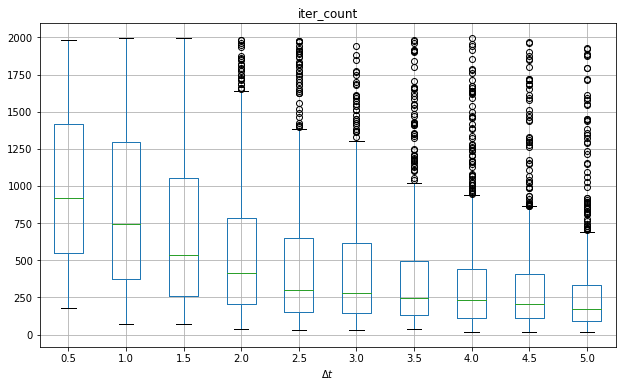
\includegraphics[scale=1,width=\textwidth]{images/brrrt_iters_high_n_3.png}
        \caption{Euclidean Distance > 30m, n=3}
    \end{subfigure}
    \begin{subfigure}[b]{0.6\textwidth}
        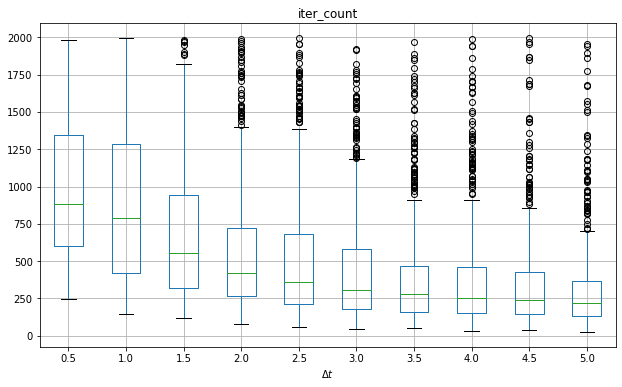
\includegraphics[scale=1,width=\textwidth]{images/brrrt_iters_high_n_6.png}
        \caption{Euclidean Distance > 30m, n=6}
    \end{subfigure}
    \caption{BR-RRT Iterations distributions for different values of $\Delta{t}$ and $n$.}
    \label{fig:brrrt_iters_high}
\end{figure}

And finally, higher value of $n$ leads to fewer failed runs. This is especially noticeable at low values of $\Delta{t}$ (Figure \ref{fig:brrrt_finish_pie_low})
and still present at higher values of $\Delta{t}$ (Figure \ref{fig:brrrt_finish_pie_high}).

\begin{figure}[H]
\centering
    \begin{subfigure}[b]{0.8\textwidth}
        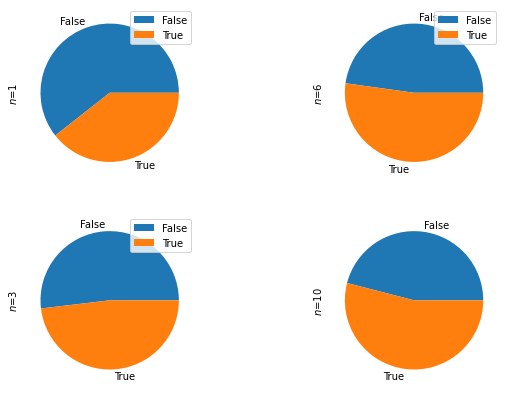
\includegraphics[scale=1.3,width=\textwidth]{images/brrrt_finish_pie_low_edge.png}
        \caption{Success/Fail at $\Delta{t}\leq 2$}
        \label{fig:brrrt_finish_pie_low}
    \end{subfigure}
    \begin{subfigure}[b]{0.8\textwidth}
        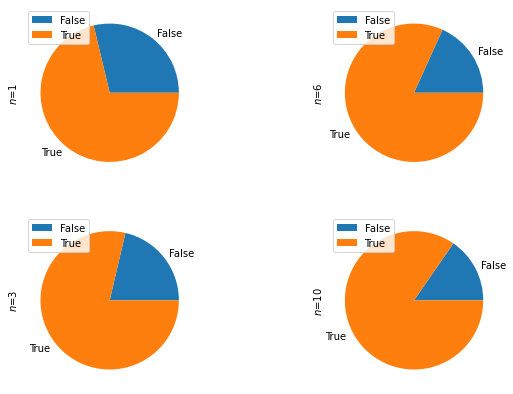
\includegraphics[scale=1.3,width=\textwidth]{images/brrrt_finish_pie_high_edge.png}
        \caption{Success/Fail at $\Delta{t} > 2$}
    \end{subfigure}
    \caption{BR-RRT Success/Fail for different values of $\Delta{t}$ and $n$.}
    \label{fig:brrrt_finish_pie_high}
\end{figure}

\section{Performance analysis}
\subsection{Sample options}
The next step was to find optimal value for sample options parameter, as the trend was already found. The algorithm was tested on 4 values for sample options parameter (1, 3, 6, 10) and 12 different start and end obstacles configurations with sample size equal to 60. That is overall sample size is equal to 2880.
\begin{figure}[H]
\begin{center}
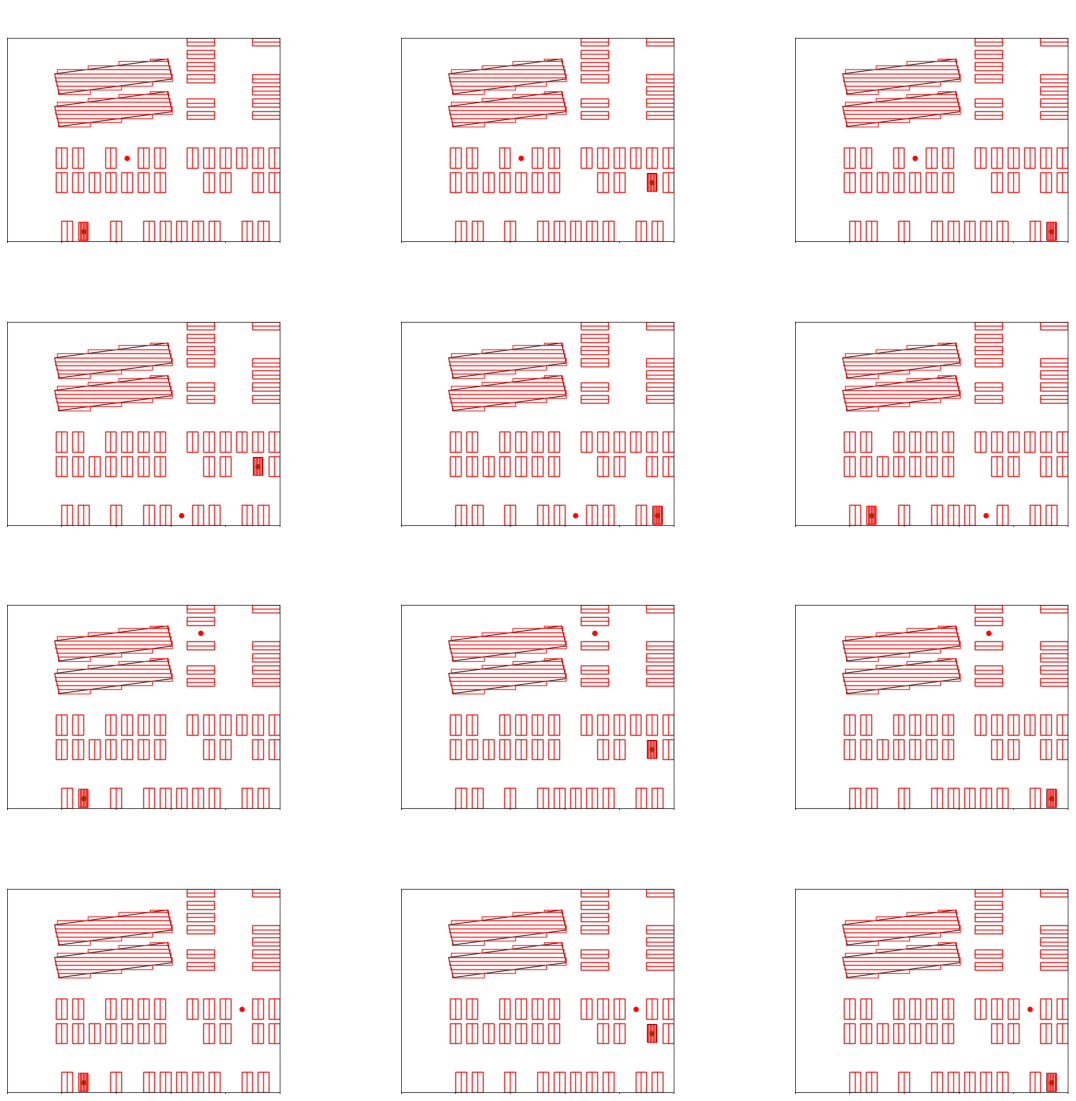
\includegraphics[scale=0.4]{images/12positions.png}
\captionsetup{width=0.6\textwidth}
\caption{12 start-end configurations selected for testing. Starting point is marked by a colored red car with a green dot, ending point is marked by a red dot.}
\end{center}
\end{figure}
Depending on the sample options value, the following plots were generated.
\begin{figure}[H]
\begin{center}
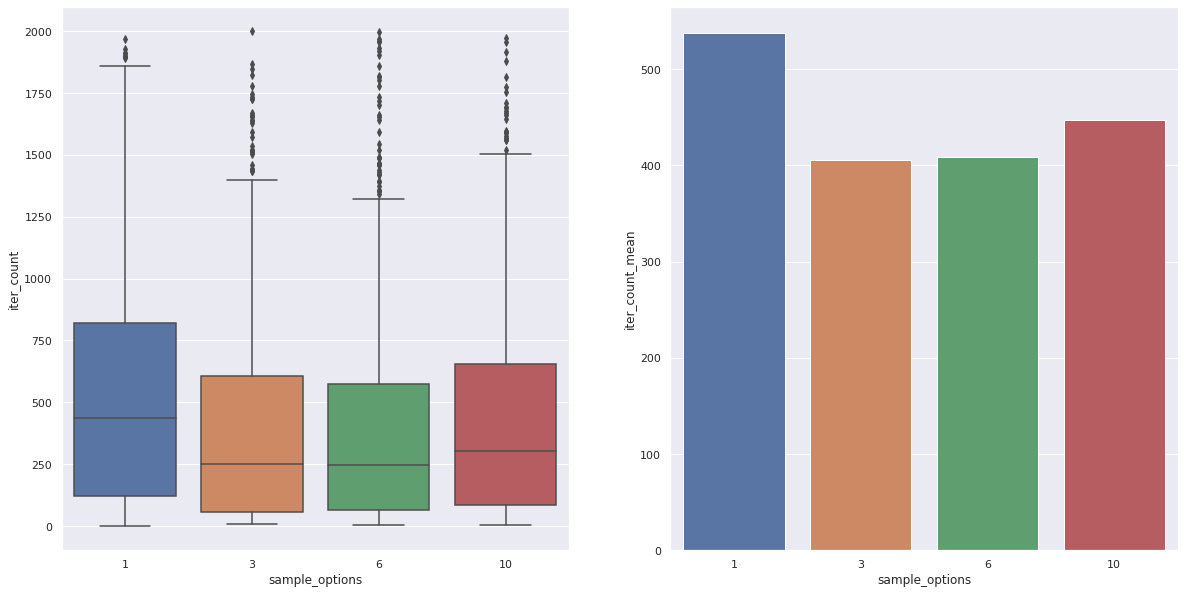
\includegraphics[scale=0.4]{images/so_iter_count.png}
\captionsetup{width=0.6\textwidth}
\caption{Distribution of number of iterations per each value of sample options.}
\end{center}
\end{figure}
Figure 5.1.2 suggests that the parameter has effect on the number of iterations the algorithm executes. The box plot (left) shows that the number of iterations tends to decrease when the number of samples is approximately between 3 and 6 (inclusive). Although the number of outliers is greater for these values than for others, this does not imply worse performance. The bar plot (right) confirms that assumption, representing the mean iterations count.
\begin{figure}[H]
\begin{center}
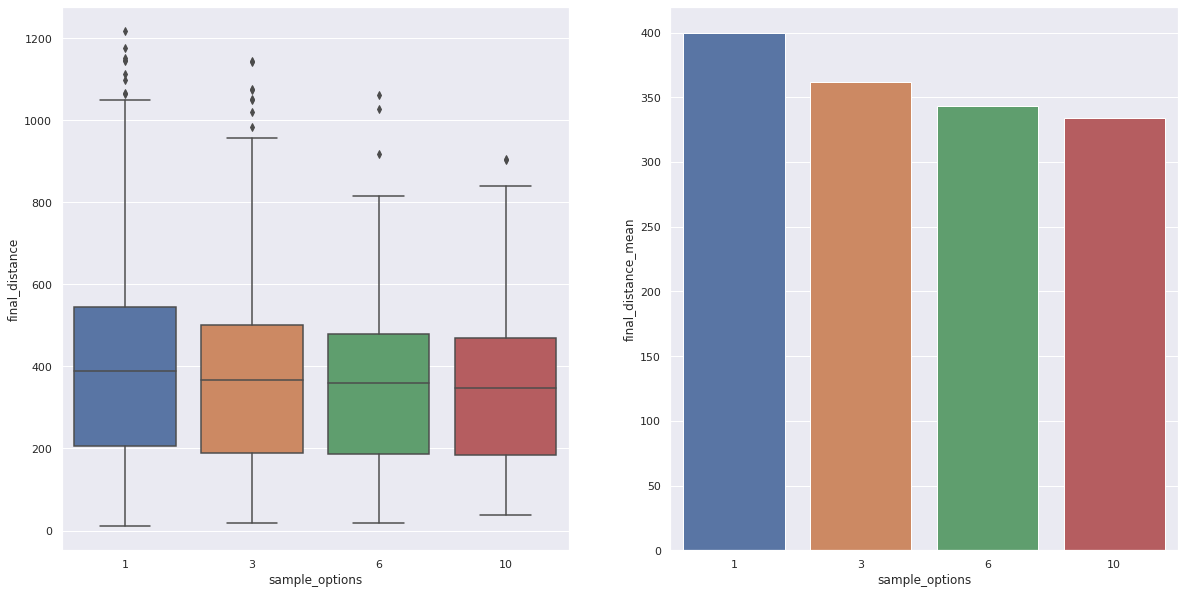
\includegraphics[scale=0.4]{images/so_final_distance.png}
\captionsetup{width=0.6\textwidth}
\caption{Distribution of final distance of a path generated by the algorithm per each value of sample options.}
\end{center}
\end{figure}
Figure 5.1.3 suggest a negative trend for final distance for increasing number of options. One possible explanation is that cardinality of options set allows RRT to create longer edges which eventually results in total distance decrease, while smaller edges often create more winding paths.
\begin{figure}[H]
\begin{center}
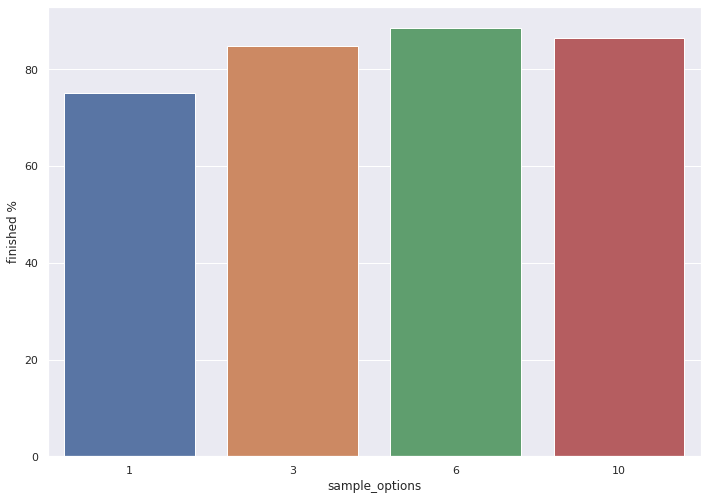
\includegraphics[scale=0.4]{images/so_finished.png}
\captionsetup{width=0.6\textwidth}
\caption{Distribution of convergence percentage of the algorithm per each value of sample options.}
\end{center}
\end{figure}
Figure 5.1.4 suggest that the sample options value has effect on the convergence rate. Similar to Figure 5.1.2 values close to 6 yield best performance.
Thus, the algorithm performance depends on the cardinality of options set. More precisely, algorithm performance peaks for parameter values close to 6.
\subsection{Start and finish points configurations}
Next, a subset containing observations with sample option parameter set to 6 was examined. The start and finish points configurations were categorized as short, medium and long based on the mean final distance. Categories are presented in Figure 5.2.1, Figure 5.2.2 and Figure 5.2.3.
\begin{figure}[H]
\begin{center}
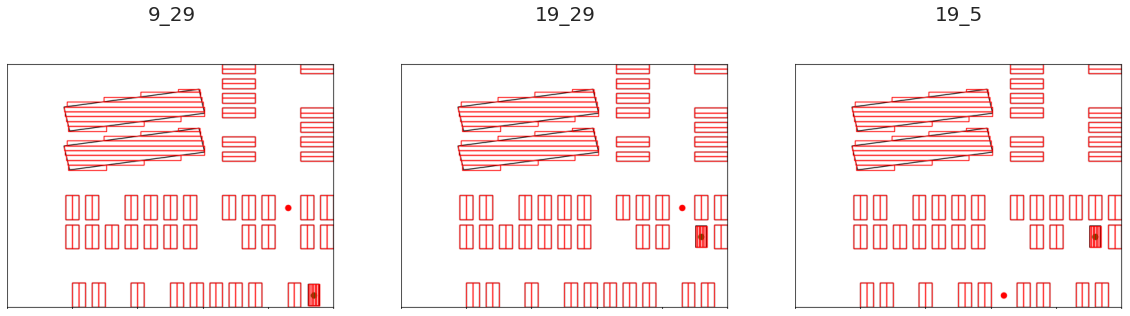
\includegraphics[scale=0.4]{images/shorts.png}
\captionsetup{width=0.6\textwidth}
\caption{Start/end configurations categorized as short.}
\end{center}
\end{figure}
\begin{figure}[H]
\begin{center}
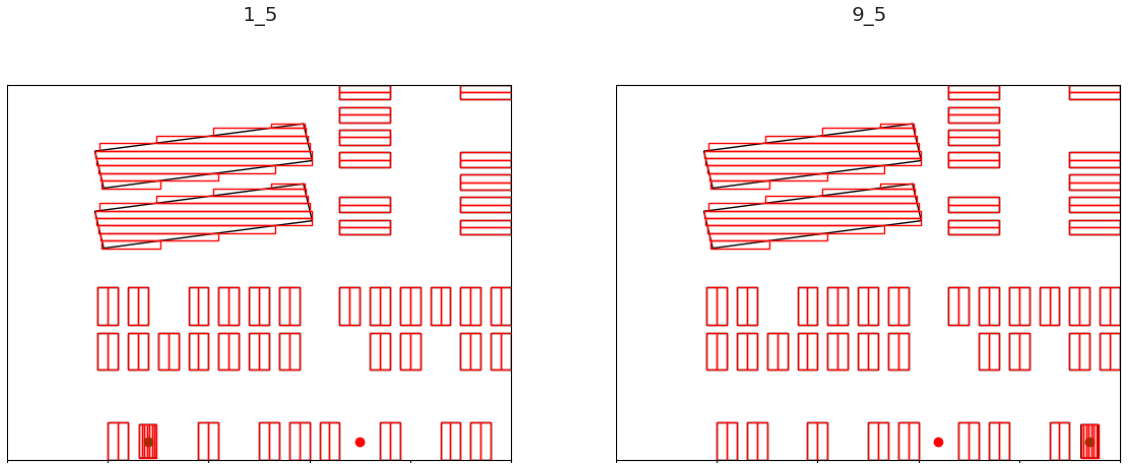
\includegraphics[scale=0.4]{images/mediums.png}
\captionsetup{width=0.6\textwidth}
\caption{Start/end configurations categorized as medium.}
\end{center}
\end{figure}
\begin{figure}[H]
\begin{center}
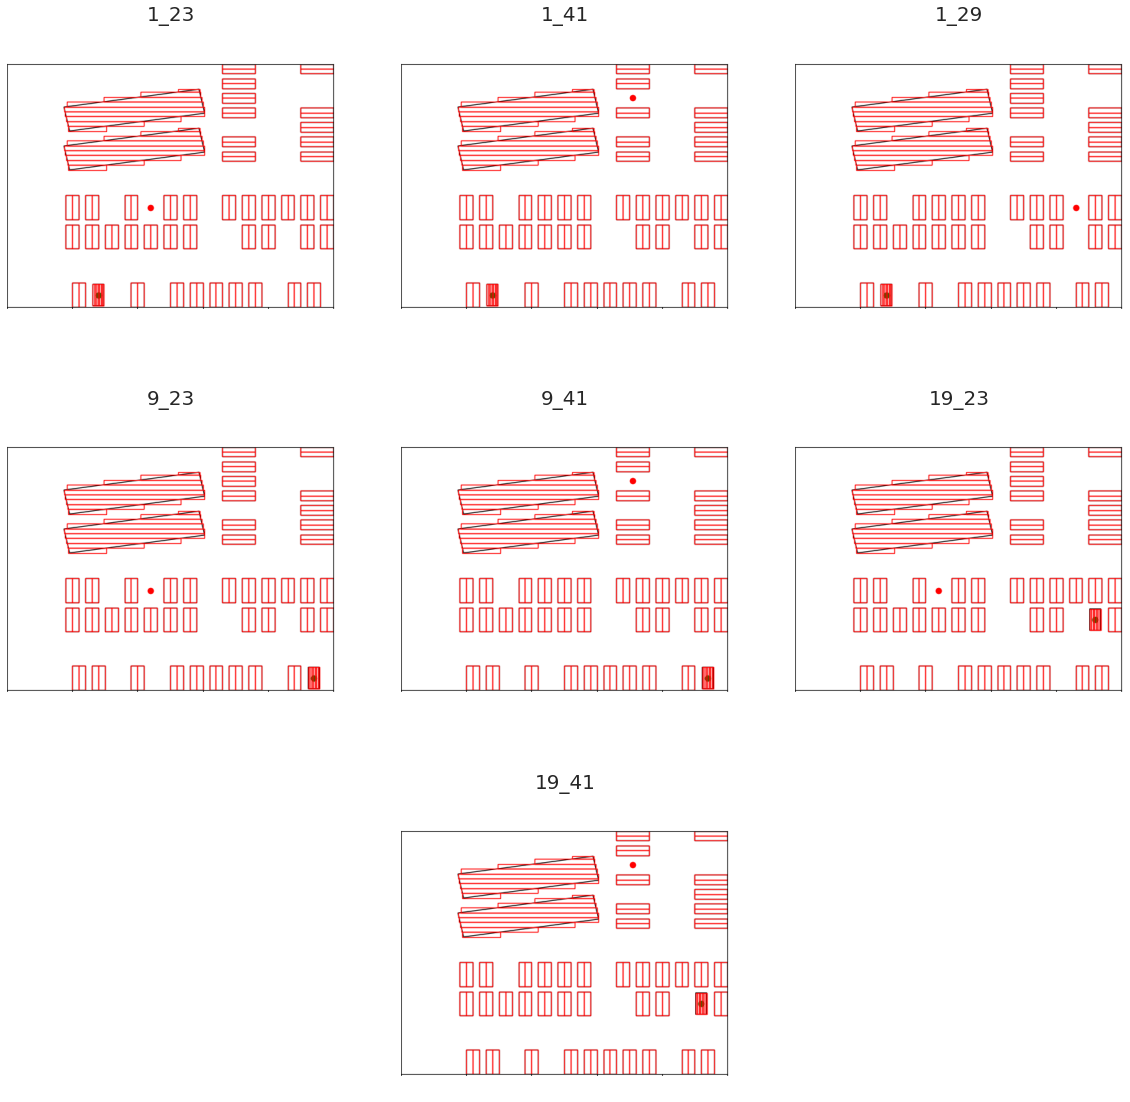
\includegraphics[scale=0.4]{images/longs.png}
\captionsetup{width=0.6\textwidth}
\caption{Start/end configurations categorized as long.}
\end{center}
\end{figure}
The algorithm showed a score of 100\% convergence rate on short and medium distances. The average convergence rate for long distances is approximately 80\%, although this parameter varies significantly among configurations of this type. More detailed data is presented in Figure 5.2.4.
\begin{figure}[H]
\begin{center}
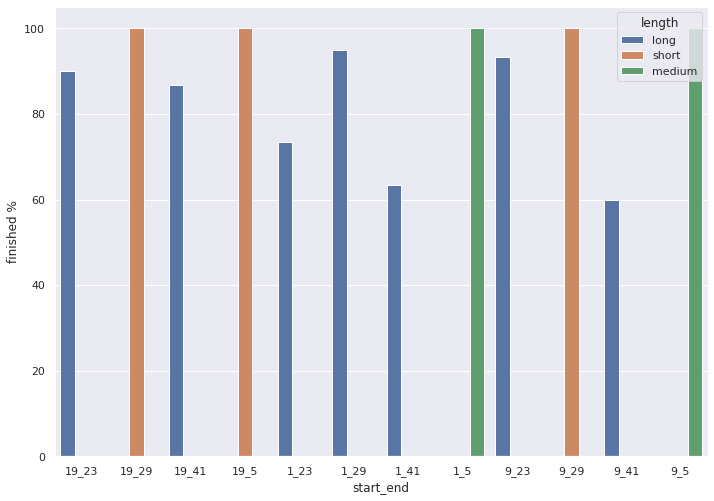
\includegraphics[scale=0.5]{images/se_finished.png}
\captionsetup{width=0.6\textwidth}
\caption{Convergence rate depending on start/end configurations.}
\end{center}
\end{figure}
The average number of iterations highly depends on the distance category, as expected. As Figure 5.2.5 suggests long paths require significantly more iterations to converge.
\begin{figure}[H]
\begin{center}
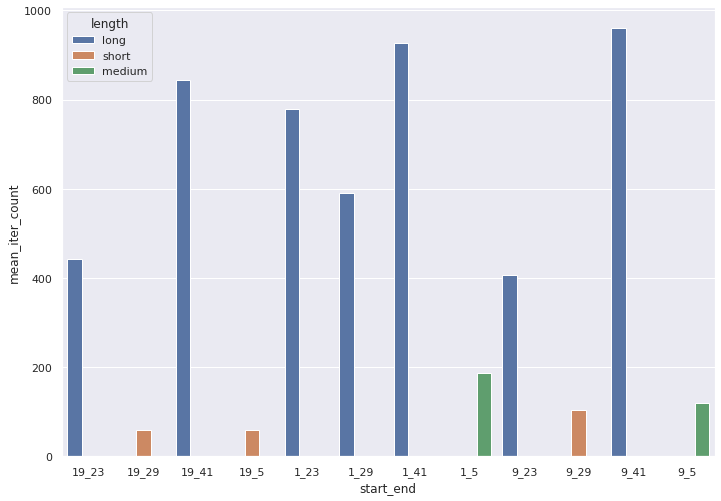
\includegraphics[scale=0.5]{images/se_iter_count.png}
\captionsetup{width=0.6\textwidth}
\caption{Mean iteration number depending on start/end configurations.}
\end{center}
\end{figure}
The pairs of points that BR-RRT struggled the most with were the ones, ending in point 41. The reason for this is that it is located in a very closed space, often making the algorithm getting stuck in narrow areas or exceeding iterations limit by exploring the whole map.

\section{Conclusion}

The algorithm BR-RRT that we have presented today, while being slightly more computationally complex, performs much better than other extensions of RRT in cluttered
environments, while creating trajectories that are guarantied to be kinodynamically and nonholonomically feasible. Unlike many other implementations it supports any-shape vehicles and is extendable with different steering functions. We have performed various tests in order to statistically find optimal parameters which
are relevant for both BR-RRT and classical RRT. There is, however, more work to be done. It is important to compare the algorithm to TP-Space based ones,
especially on low energy devices and conduct an analysis of an optimal R-Tree fan-out for both obstacles R-Tree and RRT Tree R-Tree. Improvements in R-Tree indexing
could be as low-level as page and buffer size in memory or, on a higher level, leaf and index capacities. 

\pagebreak
\section{Bibliography}

\numenum{
\item Steven M. LaValle. Planning Algorithms // Cambridge University Press. 2006. Section 4.3.1.
\item Jon Louis Bentley. Multidimensional Binary Search Trees Used for Associative Searching // Stanford University. 1975. Section 3, Section 5.
\item Sampling-based path planning with goal oriented sampling / Kang Gitae [and other] // 2016 IEEE International Conference on Advanced Intelligent Mechatronics. 2016. 1285-1290. 10.1109/AIM.2016.7576947. 
\item Sensory Steering for Sampling-Based Motion Planning / Omur Arslan [и др.] // IEEE/RSJ International Conference on Intelligent Robots and Systems. 2017. C. 3708-3715.
\item Safe and Fast Path Planning in Cluttered Environment using Contiguous Free-space Partitioning / A. K. Sadhu [and other] // 2019 International Conference on Robotics and Automation (ICRA). 2019. C. 6972-6978.
\item Search-Based Online Trajectory Planning for Car-like Robots in Highly Dynamic Environments / J. Lin [and other] // 2021 IEEE International Conference on Robotics and Automation (ICRA). 2021. С. 8151-8157.
\item TP-Space RRT – Kinematic Path Planning of Non-Holonomic Any-Shape Vehicles. Blanco, Jose Luis & Bellone, Mauro & Gimenez, Antonio // 2015. International Journal of Advanced Robotic Systems. 10.5772/60463.
\item The implementation of the BR-RRT // 2022. \href{https://github.com/Alex-Blade/KinodynamicMotionPlanning}{GitHub Repository}
}

\end{document}
